\section{نت‌کت }
نت‌کت
،یک زبان برای توصیف شبکه‌های مبتنی بر نرم‌افزار است
\cite{netkat}.
این زبان با وجود دستور زبان
\lf{Syntax}
ساده‌ای که دارد، بر اساس
KAT
\cite{kat}
بنا شده و به همین دلیل یک سیستم معادلاتی صحیح و کامل
\lf{Sound and Complete}
دارد.
این سیستم معادلاتی کمک می‌کند تا با استفاده از روش‌های جبری و اثبات تساوی برنامه‌های توصیف شده در این زبان بتوان در مورد آن‌ها استدلال کرد.

\subsection{دستور زبان نت‌کت}
در نت‌کت هر بسته
به عنوان یک نگاشت از یک مجموعه از فیلد‌های
$f_1,f_2,...,f_n$
به اعداد طبیعی با تعداد ارقام ثابت در نظر گرفته می‌شود.
آی‌پی‌
\lf{IP}
های مبدا و مقصد، نوع بسته، پورت‌
\lf{Port}
های مبدا و مقصد مثال‌هایی از این فیلد‌ها هستند.
دستور زبان نت‌کت به صورت زیر تعریف می‌شود:
\begin{align*}
    a,b ::= & 1 ~|~ 0 ~|~ f = n ~|~ a + b ~|~ a \cdot b ~|~ \neg a  \\
    p,q ::= & a ~|~ f \la n ~|~ p + q ~|~ p \cdot q ~|~ p^* ~|~ dup
\end{align*}
در این گرامر عبارت‌های
$a,b$
عملا معادل با تست‌های زبان کت
\lf{KAT}
هستند.
عبارت‌های
$p,q$
عبارت‌های نت‌کت را تعریف می‌کنند که نسبت به دستور زبان کت
جمله‌هایی به شکل
$dup$
و
$f \la n$
به آن اضافه شده است.
\begin{figure}
    \centering
    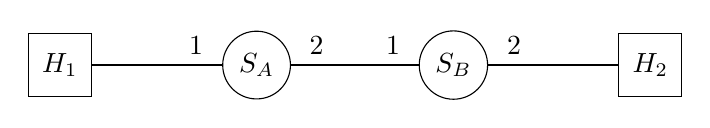
\begin{tikzpicture}[
            node distance={25mm},
            sw/.style = {draw, circle,minimum size=8mm},
            h/.style = {draw, rectangle,minimum size=8mm}
        ]
        \node[h] (h1)  {$H_1$};
        \node[sw] (sa) [right of=h1]  {$S_A$};
        \node[sw] (sb) [right of=sa] {$S_B$};
        \node[h] (h2)  [right of=sb] {$H_2$};
        \draw [thick] (h1)  -- node[above,pos=0.8]{1} (sa);
        \draw [thick] (sa) -- node[above,pos=0.2]{2}
        node[above,pos=0.8]{1}(sb);
        \draw [thick] (sb) -- node[above,pos=0.2]{2} (h2);
    \end{tikzpicture}
    \caption{مثال شبکه}
    \label{fig:netkat:ssh}
\end{figure}
برای مثال شبکه‌ی
\ref{fig:netkat:ssh}
را در نظر بگیرید که شامل دو
\lf{Switch}
A و ‌B
و دو میزبان
\lf{Host}
است.
هر سوییچ دو پورت دارد که با شماره‌های ۱ و۲ مشخص شده‌اند.
با استفاده از عبارت نت‌کت زیر می‌توانیم رفتار سوییچ‌های این شبکه را توصیف کنیم:
\begin{align}
    \label{eq:netkat:swp}
    p \triangleq (dst = H_1 \cdot pt \la 1) +
    (dst = H_2 \cdot pt \la 2)
\end{align}
این عبارت همه‌ی بسته‌هایی که مقصد آن‌ها میزبان ۱ باشد را به پورت ۱ و همه‌ی بسته‌هایی که مقصد‌ آن‌ها میزبان ۲ باشد را به پورت شماره‌ی ۲ می‌فرستد.

\subsection{مدل معنایی نت‌کت}
برای اینکه امکان استدلال در مورد مسیر‌های طی شده توسط یک بسته‌ در شبکه وجود داشته باشد،از مفهومی به نام تاریخچه‌ی بسته
\lf{Packet History}
استفاده می‌شود.
هر تاریخچه‌ی بسته‌، یک دنباله از بسته‌ها است که بسته نخست دنباله، به عنوان بسته‌ی فعلی در نظر گرفته می‌شود.
به صورت شهودی
عبارت های ۱ و ۰ به ترتیب به معنای ارسال
\lf{Forward}
و رها کردن
\lf{Drop}
بدون شرط بسته هستند.
عبارت
$f=n$
در صورتی بسته را عبور می‌دهد که مقدار فیلد
f
آن برابر با
n
باشد.
عبارت
$f \la n$
مقدار n
را به فیلد f
بسته اختصاص
می‌دهد.
عبارت‌های
$dup$
باعث می‌شوند تا یک کپی از بسته‌ی فعلی ایجاد شود و به تاریخچه‌ی بسته‌ها اضافه شود.
این عبارات در رفتار شبکه تاثیری ندارند اما امکان استدلال در مورد تمامی تغییرات ایجاد شده در حین جا‌به‌جایی بسته در شبکه را فراهم می‌سازند.
به صورت دقیق، معنای هر عبارت
\lf{Expression}
نت‌کت با استفاده از معادلات زیر تعریف می‌شود:
\begin{align}
    \sem{p}             & H \in \mathcal{P}({H}) \label{eq:netkat:sem}                  \\
    \sem{1} h           & \teq \s{h}     \label{eq:netkat:identity}                     \\
    \sem{0} h           & \teq \s{}          \label{eq:netkat:drop}                     \\
    \sem{f=n}(pk::h)    & \teq \begin{cases}
                                   \s{pk::h} & \text{ if } pk.f = n \\
                                   \s{}      & \text{ otherwise }
                               \end{cases}    \label{eq:netkat:filter}                  \\
    \sem{\neg a}h       & \teq \s{h} \setminus (\sem{a}h) \label{eq:netkat:nfilter}     \\
    \s{f \la n} (pk::h) & \teq \s{pk[f:=n]::h}     \label{eq:netkat:assign}             \\
    \sem{p+q}h          & \teq \sem{p}h \cup \sem{q}h   \label{eq:netkat:sum}           \\
    \sem{p\cdot q} h    & \teq (\sem{p} \bullet \sem{q}) h    \label{eq:netkat:dot}     \\
    \sem{p^*}h          & \teq \bigcup_{i \in \mathbb{N}}F^i h \label{eq:netkat:kleene} \\
    F^0 h               & \teq \s{h}                                                    \\
    F^{i+1} h           & \teq (\sem{p} \bullet F^i) h                                  \\
    (f \bullet g) x     & \teq \bigcup\s{g(y)|y \in f(x)}                               \\
    \sem{dup} (pk::h)   & \teq \s{pk::(pk::h)} \label{eq:netkat:dup}
\end{align}
در معادلات بالا فرض می‌شود که
$H$
مجموعه‌ی تمامی تاریخچه‌های ممکن است.
معادله‌ی
\ref{eq:netkat:sem}
بیان می‌کند که معنی هر عبارت نت‌کت روی یک تاریخچه‌ی بسته یک مجموعه از
تاریخچه‌ی بسته‌های حاصل از اعمال این عبارت روی تاریخچه‌ی ورودی است.
معادله‌ی
\ref{eq:netkat:identity}
بیان می‌کند که عبارت ۱ بسته را بدون شرط عبور می‌دهد.
در مقابل معادله‌ی
\ref{eq:netkat:drop}
رها شدن بسته را با خروجی یک مجموعه‌ی خالی مدل می‌کند.
معادله‌ی
\ref{eq:netkat:filter}
بسته‌ی نخست ورودی را بررسی می‌کند و اگر مطابق با عبارت نبود بسته رها می‌شود.
نقیض یک فیلتر در معادله‌ی
\ref{eq:netkat:nfilter}
توصیف شده است.
معادله‌ی
\ref{eq:netkat:assign}
مقدار
$n$
را به فیلد
$f$
بسته‌ی نخست تاریخچه اختصاص می‌دهد.
معادله‌ی
\ref{eq:netkat:sum}
جمع دو جمله را به صورت اجتماع تاریخچه‌های حاصل از اعمال هر یک از عملوند‌ها توصیف می‌کند.
در معادله‌ی
\ref{eq:netkat:dot}
ترکیب متوالی دو جمله را به صورت ترکیب
Kleisli
دو جمله که به شکل زیر تعریف می‌شود توصیف می‌کند:
\begin{align*}
    (f \bullet g) x \triangleq \bigcup \s{g\ y ~|~ y \in f\ x}
\end{align*}
در معادله‌ی
\ref{eq:netkat:kleene}
حاصل اپراتور ستاره‌ی کلینی
\lf{Kleene Star}
معادل با اجتماع اعمال تابع‌های
$F_i$
روی تاریخچه‌ی ورودی در نظر گرفته شده است که تابع
$F_i$
حاصل
$i$
بار
ترکیب
Kleisli
عبارت
$p$
است.
در نهایت معادله‌ی
\ref{eq:netkat:dup}
یک کپی از بسته‌ی نخست ورودی را به ابتدای خروجی اضافه می‌کند.

نت‌کت علاوه بر اصول موضوعه‌ی
\lf{Axiom}
KAT
اصول‌ موضوعه‌ی زیر را هم شامل می‌شود تا دستگاه معادلاتی صحیح و کامل
\lf{Sound and Complete}
داشته باشد:
\begin{align}
    f \la n \cdot f' \la n' & \equiv f' \la n' \cdot f \la n,
    \text{ if } f \neq f' \label{mod-mod-comm}
    \\
    f \la n \cdot f' = n'   & \equiv f' = n' \cdot f \la n,
    \text{ if } f \neq f' \label{mod-filter-comm}                            \\
    dup \cdot f = n         & \equiv f = n \cdot dup \label{dup-filter-comm} \\
    f \la n \cdot f = n     & \equiv f \la n \label{mod-filter}              \\
    f = n \cdot f \la n     & \equiv f = n \label{filter-mod}                \\
    f \la n \cdot f \la n'  & \equiv f \la n' \label{mod-mod}                \\
    f = n \cdot f = n'      & \equiv 0, \text{ if } n \neq n' \label{contra} \\
    \Sigma_{i} f = i        & \equiv 1 \label{match-all}
\end{align}
اصل‌های
\ref{mod-mod-comm},\ref{mod-filter-comm},\ref{dup-filter-comm}
خواص جابه‌جایی
\lf{Commutative}
عملیات‌ها را بیان می‌کنند.
اصل
\ref{mod-filter}
بیان می‌کند که اختصاص مقدار
n
به یک فیلد و سپس  فیلتر کردن بر روی این فیلد با همین مقدار معادل با عملیات اختصاص
\lf{Assignment}
به تنهایی است.
مشابه همین اصل برای یک فیلتر و سپس یک اختصاص هم در اصل
\ref{filter-mod}
مشخص شده.
اصل
\ref{mod-mod}
بیان می‌کند که در دنباله‌ای از اختصاص مقادیر به یک فیلد مشخص، تنها آخرین اختصاص تاثیر دارد.
در اصل
\ref{contra}
مشخص شده است که مقدار یک فیلد نمی‌تواند دو مقدار متفاوت داشته باشد.
در نهایت اصل
\ref{match-all}
بیان می‌کند که عملیات مجموع فیلتر‌ها به ازای هر مقدار ممکن برای یک فیلد مشخص برابر عنصر همانی
\lf{Identity}
است.

\subsection{توصیف رفتار شبکه با نت‌کت}
در ادامه فرض کنید که بخواهیم شبکه‌ای مانند شکل
\ref{fig:netkat:ssh}
را توصیف کنیم که در آن بسته‌هایی که از نوع
SSH
هستند اجازه‌ی عبور نداشته باشند.
همچنان می‌توانیم از سیاست توصیف شده توسط
\ref{eq:netkat:swp}
برای توصیف رفتار سوییچ‌ها استفاده کنیم.
در ادامه می‌توان با اضافه کردن یک فیلتر به این عبارت، ویژگی دسترسی کنترل
\lf{Access Control}
را به این سیاست اضافه کرد تا همه‌ی بسته‌های از نوع
SSH
را رها کند:
\begin{align*}
    p_{AC} \triangleq \neg(typ = SSH)\cdot p
\end{align*}
اما استفاده از عبارت بالا به تنهایی برای توصیف رفتار شبکه شکل
\ref{fig:netkat:ssh}
کافی‌ نیست.
برای تکمیل این عبارت لازم است تا رفتار توپولوژی
\lf{Topology}
شبکه‌ هم به آن افزوده شود.
در نت‌کت توپولوژی شبکه به عنوان یک گراف جهت‌دار در نظر گرفته می‌شود و رفتار آن در قالب اجتماع رفتار هر یک از پیوندهای
\lf{Link}
آن توصیف می‌شود.
برای شبکه‌ی شکل
\ref{fig:netkat:ssh}
می‌توان از عبارت زیر برای توصیف توپولوژی شبکه استفاده کرد:
\begin{align*}
    t \triangleq & (sw = A \cdot pt = 2 \cdot sw \la B \cdot pt \la 1) + \\
                 & (sw = b \cdot pt = 1 \cdot sw \la A \cdot pt \la 2) + \\
                 & (sw = b \cdot pt = 2)
\end{align*}
در نت‌کت در صورتی که سیاست و توپولوژی شبکه در قالب عبارت‌هایی توصیف شده‌باشند،
رفتار کل شبکه در واقع دنباله‌ای از اعمال این عبارت‌ها به صورت یکی در میان است.
به عنوان مثال در شکل
\ref{fig:netkat:ssh}
یک بسته از میزبان ۱ ابتدا توسط سوییچ
A
پردازش شده، سپس روی لینک بین دو سوییچ جا به جا می‌شود و در نهایت توسط سوییچ
B
پردازش می‌شود.
در نت‌کت می‌توان این رفتار را به صورت
$p_{AC}\cdot t \cdot p_{AC}$
توصیف کرد.
با استفاده از همین شهود، رفتار کل شبکه را می‌توان در قالب عبارت زیر توصیف کرد:
\begin{align*}
    (p_{AC}\cdot t)^*
\end{align*}
در توصیف بالا فرض شده است که بسته‌ها می‌توانند به هر طریق ممکن وارد شبکه و از آن خارج شوند، اما این رفتار همیشه مورد قبول نیست.
به عنوان مثال در شبکه شکل
\ref{fig:netkat:ssh}
اگر مکان‌های ورودی و خروجی شبکه را در قالب عبارت زیر توصیف کنیم:
\begin{align*}
    e \triangleq sw = A\cdot port = 1 \vee sw = B \cdot port = 2
\end{align*}
می‌توانیم رفتار انتها به انتهای
\lf{End to End}
شبکه را به شکل زیر توصیف کنیم:
\begin{align*}
    p_{net} \triangleq e \cdot (p_{AC}\cdot t)^* e
\end{align*}
در حالت کلی‌تر، نیازی به توصیف ورودی و خروجی‌های شبکه در قالب یک عبارت نیست.
پس اگر فرض شود که مکان‌های ورودی شبکه توسط عبارت
$in$
و مکان‌های خروجی شبکه در قالب عبارت
$out$
توصیف شده‌ باشند، رفتار یک شبکه در نت‌کت به صورت زیر تعریف می‌شود:
\begin{align*}
    in \cdot (p\cdot t)^*\cdot out
\end{align*}
که عبارت
$p$
سیاست شبکه و عبارت
$t$
توپولوژی شبکه است.

\subsection{درستی‌سنجی برنامه‌های نت‌کت}
درستی‌سنجی یک شبکه و بررسی خواص آن در نت‌کت با استفاده از بررسی تساوی عبارت یک شبکه با عبارت‌های دیگر انجام می‌شود.
به عنوان مثال در شبکه‌ی شکل
\ref{fig:netkat:ssh}
برای بررسی اینکه همه‌ی بسته‌ها با نوع
SSH
از میزبان ۱ رها می‌شوند کافی است تا تساوی زیر را ثابت کنیم:
\begin{equation*}
    \begin{pmatrix}
        type = SSH \cdot sw = A \cdot pt = 1 \cdot \\
        (p_{AC}\cdot t) ^ * \cdot                  \\
        sw = B\cdot pt = 2
    \end{pmatrix}
    \equiv 0
\end{equation*}
از طرفی برای بررسی یک خاصیت در شبکه، مثلا امکان فرستاده شدن‌ همه‌ی بسته‌هایی که از نوع
SSH
نیستند از میزبان ۱ به میزبان ۲
می‌توان به جای بررسی تساوی دو عبارت از نامساوی
$p \leq q$
استفاده کرد.
این نامساوی که خلاصه شده‌ی تساوی
$p + q \equiv q$
است بیان می‌کند که رفتار عبارت
$p$
بخشی از رفتار عبارت
$q$
است.
بنابراین برای بررسی این مساله که شبکه‌ی شکل
\ref{fig:netkat:ssh}
بسته‌های غیر
$SSH$
از میزبان ۱ را عبور می‌دهد کافی است تا درستی نامعادله‌ی زیر را بررسی کرد:
\begin{equation*}
    \begin{pmatrix}
        \neg(type = SSH) \cdot sw = A \cdot pt = 1 \cdot & \\
        sw \la B \cdot pt \la 2                          &
    \end{pmatrix}
    \leq (p_{AC}\cdot t)^ *
\end{equation*}
اصول موضوعه‌ی نت‌کت یک سیستم اثبات
\lf{Proof System}
را تشکیل می‌دهند که امکان اثبات این معادله یا نامعادله‌ها را فراهم می‌کنند.
مثلا فرض کنید که سیاست دسترسی‌کنترل برای رها کردن بسته‌های
SSH
\ref{fig:netkat:ssh}
را برای افزایش کارایی فقط در سوییچ
A
انجام دهیم:
\begin{align*}
    p_A \triangleq (sw = A \cdot \neg(typ = \texttt{SSH})\cdot p)
    + (sw = B \cdot p)
\end{align*}
به طریق مشابه می‌توانیم این کار را در سوییچ
B
هم انجام دهیم:
\begin{align*}
    p_B (sw = A\cdot p) \triangleq (sw = B \cdot \neg(typ = \texttt{SSH})\cdot p)
\end{align*}
فرض کنید مکان‌های ورودی و خروجی به صورت زیر تعریف شده باشند:
\begin{align*}
    in  & \triangleq (sw = A \cdot pt = 1) \\
    out & \triangleq (sw = B \cdot pt = 2)
\end{align*}
اثبات معادل بودن دو سیاست
$p_A$
و
$p_B$
بر اساس این ورودی و خروجی در شکل
\ref{fig:netkat:proof}
ذکر شده است.

\begin{figure}
    \centering
    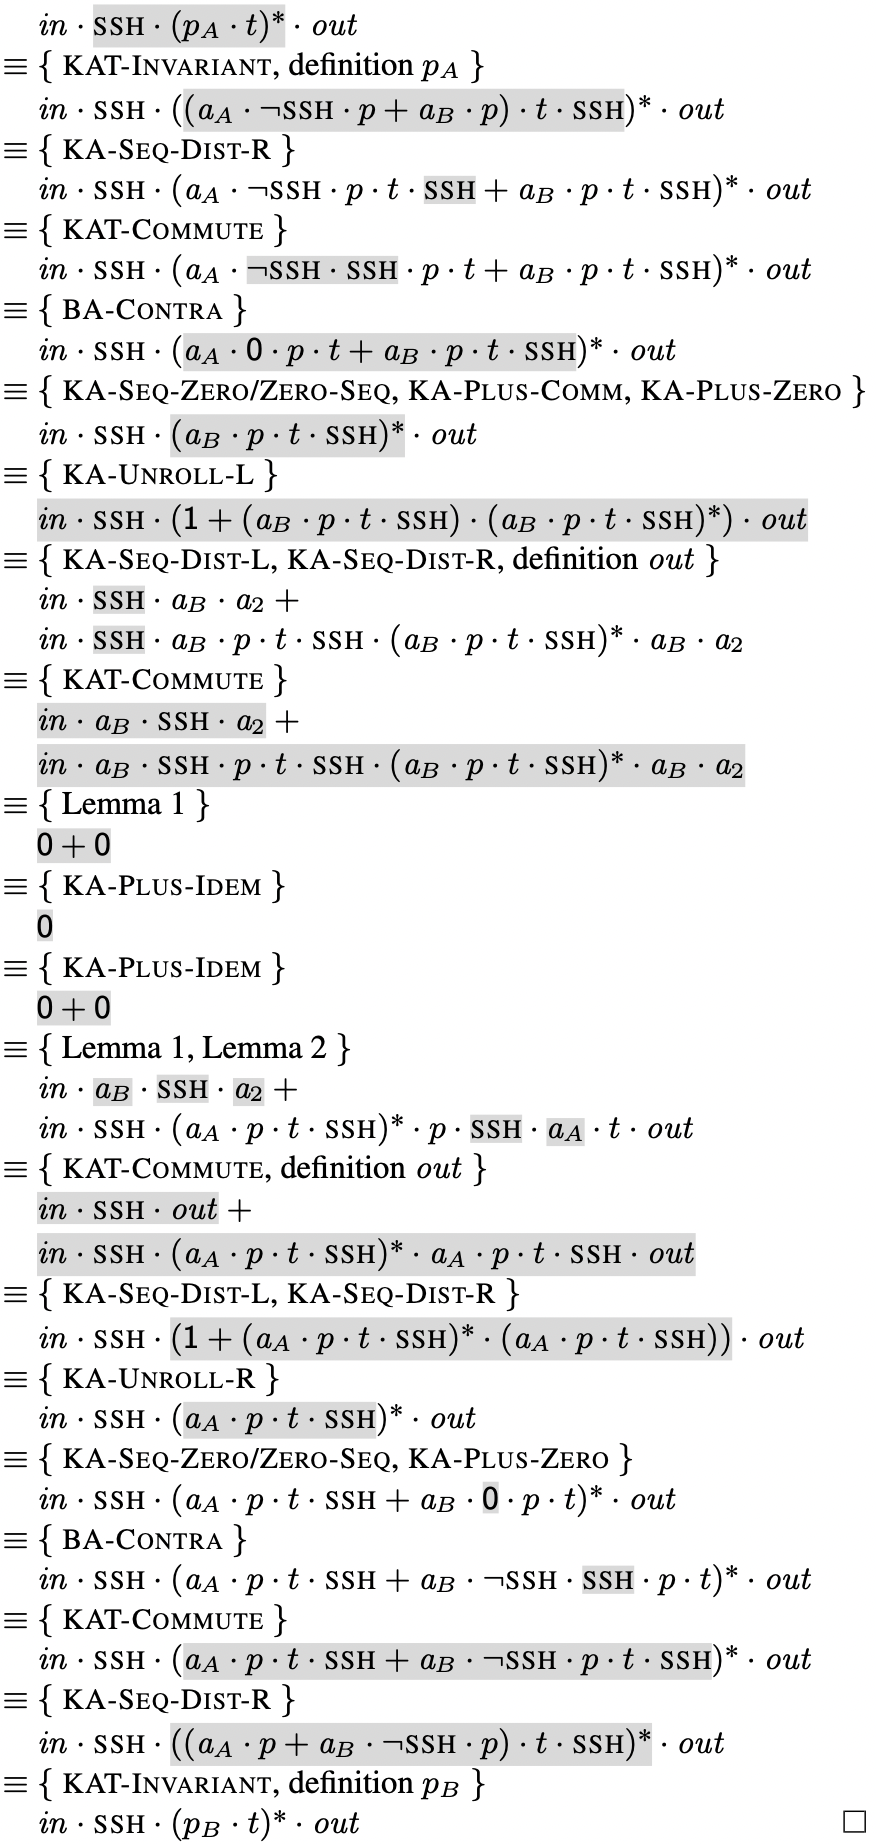
\includegraphics[width=10cm]{proof.png}
    \caption{اثبات معادل بودن
        $p_A$
        و
        $p_B$
        \cite{netkat}
    }
    \label{fig:netkat:proof}
\end{figure}